% 11-45 pages (27 on average)
% aim for 2-5 pages for each major section
\chapter{Background}

TODO: outside of specific sections, have a one-paragraph introduction before and a one-paragraph summary at the end.

\section{Propositional Logic} \label{sec:proplogic}

In this section, we briefly introduce the fundamentals of propositional logic and describe some logic-based computational problems. We refer the reader to the book by \cite{DBLP:books/daglib/0029942} for a more detailed introduction to logic and its role in computer science.

An \emph{atomic proposition} (also known as \emph{atom} and Boolean/logical variable) is a variable with two possible (truth) values: true and false. Unless specified otherwise, we will refer to atoms as \emph{variables}. A \emph{formula} is any well-formed expression that connects variables using the following Boolean/logical operators (and parentheses): negation ($\neg$), disjunction ($\lor$), conjunction ($\land$), (material) implication ($\Rightarrow$), and equivalence (i.e., material biconditional) ($\Leftrightarrow$). A \emph{literal} is either a variable or its negation, respectively called \emph{positive} and \emph{negative} literal. A \emph{clause} is a disjunction of literals.\footnote{In the context of logic programs, the word \emph{clause} is used differently (see \cref{sec:lp,chapter:randomlps}).} A formula is in \emph{conjunctive normal form} (CNF) if it is a conjunction of clauses, and it is in $k$-CNF if every clause has exactly $k$ literals. Many other normal forms and ways to represent propositional formulas are covered in \cref{sec:kc}.

An \emph{interpretation} (also known as a \emph{variable assignment}) of a formula $\phi$ is a map from the variables of $\phi$ to the set $\{\, \text{true}, \text{false} \,\}$. A \emph{model} is an interpretation under which $\phi$ evaluates to true. A formula is \emph{satisfiable} if it has at least one model.

Throughout the thesis, we use set-theoretic notation for many concepts in logic such as clauses and formulas in CNF (e.g., we write $c \in \phi$ to mean that clause $c$ is one of the clauses of formula $\phi$). However, this does not automatically mean that we assume no duplicates---whether or not that is the case is clarified on a case-by-case basis.

\begin{example} \label{example:logic}
  Formula $\phi \coloneqq (\neg a \lor b) \land a$ has two variables $a$ and $b$, is in CNF, and contains two clauses. The first clause $\neg a \lor b$ has a negative literal $\neg a$ and a positive literal $b$. Since $\phi$ has two variables, it also has four interpretations. Interpretation $\{\, a \mapsto \text{true}, b \mapsto \text{true} \,\}$ is a model, so $\phi$ is satisfiable. An equivalent set-theoretic representation of $\phi$ is $\{\, \{\, \neg a, b \,\}, \{\, a \,\} \,\}$.
\end{example}

\subsection{Logic-Based Computational Problems} \label{sec:logicproblems}

We begin with a description of \SAT{} and some of its extensions. Given a propositional formula\footnote{Unless stated otherwise, formulas for \SAT{} and other similar problems are assumed to be in CNF.}, \SAT{} asks whether the formula is satisfiable. \SAT{} (also known as \emph{propositional/Boolean satisfiability}) is the first problem shown to be \NP-complete \citep{DBLP:conf/stoc/Cook71,levin1973universal}. Motivated by many real-life problems that were found to be reducible to \SAT{}, research in \SAT{} solving produced algorithms that can efficiently tackle large instances despite the exponential worst-case time complexity \citep{DBLP:series/faia/2009-185}.

Instead of satisfying all clauses, one can attempt to find an interpretation that satisfies the maximum number of clauses---this problem is called Max\SAT{} \citep{bacchus2021maximum,DBLP:series/faia/LiM09}. It is an \NP-hard optimisation problem that (in its most general form) attaches a (potentially infinite) cost for failing to satisfy each clause and seeks to minise total cost.

\#\SAT{}, or \emph{(propositional) model counting}, asks to count the number of models of a formula \citep{DBLP:series/faia/GomesSS09}. \#\SAT{} is the canonical \#\P-complete problem with many applications in areas such as planning and probabilistic reasoning. $\#\exists\SAT{}$, or \emph{projected model counting}, selects a subset of variables called \emph{priority variables} \citep{DBLP:conf/sat/AzizCMS15}. The task is then to count the number of assignments of values to priority variables that can be extended to models. The extension of \#\SAT{} most relevant to our work is called \emph{weighted model counting} (WMC). Given a propositional formula $\phi$ and a \emph{weight function} $w$ from the literals of $\phi$ to non-negative real numbers, WMC asks to compute
\[
\mathrm{WMC}(\phi) = \sum_{\omega \models \phi} \prod_{\omega \models l} w(l),
\]
where the summation is over all models $\omega$ of $\phi$, and the product is over all literals of $\omega$ \citep{DBLP:journals/ai/ChaviraD08}. Lastly, both \#\SAT{} and WMC have been extended to first-order logic \citep{DBLP:conf/ijcai/BroeckTMDR11}---this is the topic of \cref{chapter:wfomc}.

\begin{example} \label{example:wmc1}
  The model count of the formula in \cref{example:logic} is equal to one. With a weight function $w \coloneqq \{\, a \mapsto 0.7, \neg a \mapsto 0.2, b \mapsto 0.8, \neg b \mapsto 0.7 \,\}$, the WMC of the same formula is $0.7 \times 0.8 = 0.56$.
\end{example}

\begin{example}
  With the same weight function $w$ as in \cref{example:wmc1}, the WMC of formula $a \lor b$ is $w(a)w(b) + w(a)w(\neg b) + w(\neg a)w(b) = 0.7 \times 0.8 + 0.7 \times 0.7 + 0.2 \times 0.8 = 1.21$, and the model count of this formula is 3.
\end{example}

There are a number of other computational problems that similarly use logical or algebraic constructs to encode problems from various domains. First, a propositional formula with prepended quantifiers for all of its variables is known as a \emph{quantified Boolean formula} \citep{DBLP:series/faia/BuningB09}. One can then ask whether the formula is true or false. \emph{Satisfiability module theories} considers \SAT{} in the context of a background theory \citep{DBLP:series/faia/BarrettSST09}. These theories can describe the properties of integer arithmetic, sets, trees, strings, and many commonly-used abstract data structures. \emph{Pseudo-Boolean} solvers consider decision and optimisation problems that can be expressed as linear inequalities over Boolean variables \citep{DBLP:series/faia/RousselM09}. \emph{Integer (linear) programming} instances encode integer optimisation problems under inequality constraints of a certain linear-algebraic form \citep{wolsey2020integer}. Finally, \emph{constraint programming} is a powerful paradigm for solving combinatorial search and optimisation problems with a much more expressive syntax \citep{DBLP:reference/fai/2}---we discuss constraint programming in more detail in \cref{sec:cp}.

\section{Declarative Programming}

In a declarative programming language, one describes \emph{what} is to be computed but not \emph{how}. Here we describe two declarative programming paradigms pertinent to our work: logic programming and constraint programming.

\subsection{Logic Programming} \label{sec:lp}

In this subsection, we give a brief introduction to logic programming. Specifically, we focus on Prolog---the most popular logic programming language to date. We do not, however, attempt to cover all (or even most) of the capabilities of Prolog but rather focus on the main concepts and ideas relevant to our work in \cref{chapter:randomlps}. Note that different descriptions of logic programming often use different (and mutually inconsistent) terminologies. Here we prioritise names and definitions that are sufficiently general for our needs and reasonably consistent with the terminology used in logic. For more details on logic programming and Prolog, we refer the reader to some of the numerous books on the subject \citep{DBLP:books/daglib/0041598,DBLP:books/daglib/0067951}.

A \emph{logic program} is a finite sequence\footnote{Although it is common to define logic programs as sets, the order is important for efficiency and can be the difference between finite and infinite running time.} of clauses. A \emph{clause} consists of a head and a body. If a clause has an empty body, it is a \emph{fact}, otherwise it is a \emph{rule}. The Prolog syntax for a fact and a rule is \verb+h.+ and \verb+h :- b.+, respectively, where \texttt{h} is the head and \texttt{b} is the body, although we often write $\texttt{h} \gets \texttt{b}$ instead.

The \emph{head} of a clause is an atom. An \emph{atom} (i.e., atomic formula) has the form $p(t_1, \dots, t_n)$, where $p$ is a \emph{predicate (symbol)}, and $(t_i)_{i=1}^n$ are terms. Here, $n \in \mathbb{N}_0$ is the \emph{arity} of $P$. Some built-in predicates such as equality can be written in infix notation and without parentheses, i.e., as $a = b$ instead of $=(a, b)$. A \emph{term} is either a \emph{(logical) variable} (i.e., a string that begins with a capital letter) or a \emph{constant} (i.e., any other string).

The \emph{body} of a clause is a formula.\footnote{In the literature, it is common to define clause bodies as conjunctions, but here we present a more general definition, given that such a generalisation is widely supported by the relevant software.} A \emph{formula} is any well-formed expression that connects atoms using conjunction, disjunction, and negation (as well as parentheses). Prolog syntax for these operators is different from the standard notation used in logic: we write `\verb+,+' instead of $\land$, `\verb+;+' instead of $\lor$, and `\verb#\+#' instead of $\neg$. Just like with the syntax for clauses, in most cases we continue to use logic-based syntax for convenience.

Finally, a \emph{query} is a formula to be evaluated. If the query has no variables, the evaluation returns either true or false. Otherwise, the logic programming engine tries to replace the variables of the query with constants such that the resulting formula is a logical consequence of the program. If successful, an example of such a mapping is returned; if not, the engine returns false.

\begin{example}
  Consider the following logic program.
\begin{verbatim}
parent(sky, will).
parent(will, zoe).
ancestor(X, Z) :- parent(X, Z); (parent(X, Y), ancestor(Y, Z)).
\end{verbatim}
In our alternative logic-based notation, the last clause could also be written as
\[
\texttt{ancestor(X, Z)} \gets \texttt{parent(X, Z)} \lor (\texttt{parent(X, Y)} \land \texttt{ancestor(Y, Z)}).
\]

This program has three clauses. The first two clauses are facts whereas the last clause is a rule. The program uses two predicates (\texttt{parent} and \texttt{ancestor}), three constants (\texttt{sky}, \texttt{will}, and \texttt{zoe}), and the last clauses uses three variables (\texttt{X}, \texttt{Y}, and \texttt{Z}). Both predicates are of arity 2.

Clause-by-clause, this program can be interpreted as:
\begin{itemize}
\item Sky is a parent of Will.
\item Will is a parent of Zoe.
\item \texttt{X} is an ancestor of \texttt{Z} if \texttt{X} is a parent of \texttt{Z} or there is a \texttt{Y} such that \texttt{X} is a parent of \texttt{Y}, and \texttt{Y} is an ancestor of \texttt{Z}.
\end{itemize}

The query \texttt{ancestor(sky, zoe)} returns true since Sky is a parent of a parent of Zoe, and thus an ancestor. The query \texttt{ancestor(X, sky)} returns false because we know nothing about the ancestors of Sky. Lastly, the query \texttt{ancestor(sky, X)} could return either $\{\, \texttt{X} \mapsto \texttt{will} \,\}$ or $\{\, \texttt{X} \mapsto \texttt{zoe} \,\}$ as both Will and Zoe have Sky as an ancestor.
\end{example}

% TODO: could also describe stratification in more detail (either here or in Chapter 3)
%% \paragraph{Things to mention.}
%% \begin{itemize}
%% \item we're not defining literals here
%% \item the generalisation of clauses affects the definitions of stratification and dependency graph as well
%% \item Stratification
%%   \begin{itemize}
%%   \item \emph{Stratification} is a condition necessary for probabilistic logic programs
%%     \citep{DBLP:conf/padl/MantadelisR17} and often enforced on logic programs
%%     \citep{DBLP:journals/tcs/Bidoit91} that helps to ensure a unique answer to every
%%     query. This is achieved by restricting the use of negation so that any program
%%     $\mathscr{P}$ can be partitioned into a sequence of programs $\mathscr{P} =
%%     \bigsqcup_{i=1}^n \mathscr{P}_i$ such that, for all $i$, the negative literals
%%     in $\mathscr{P}_i$ can only refer to predicates defined in $\mathscr{P}_j$ for
%%     $j \le i$ \citep{DBLP:journals/tcs/Bidoit91}.
%%   \item include the formal definition from the original paper \citep{DBLP:books/mk/minker88/AptBW88}
%%   \item also include a good example
%%   \item consider including the definition of a (predicate) dependency graph and the lemma that follows. I think the original definition is slightly different: it allows edges to be positive and negative at the same time.
%%   \item (the original paper) shown that stratified programs are always consistent (i.e., avoid paradoxical situations such as $p \gets \neg p$) \citep{DBLP:books/mk/minker88/AptBW88}
%%   \item only a sufficient condition for consistency
%%   \end{itemize}
%% \end{itemize}

\subsection{Constraint Programming} \label{sec:cp}

Constraint models are successfully used to tackle search problems in many domains such as bioinformatics, configuration, networks, planning, scheduling, and vehicle routing \citep{DBLP:reference/fai/2}. Here we briefly describe what a constraint satisfaction problem (CSP) is, how an algorithm might attempt to solve it, and how one can help the algorithm search efficiently.

\begin{definition}
  A \emph{CSP} is a triple $(X, D, C)$, where
  \begin{itemize}
  \item $X = (x_i)_{i=1}^n$ is an $n$-tuple of variables,
  \item $D = (D_i)_{i=1}^n$ is an $n$-tuple of (typically, finite) domains such that $x_i \in D_i$,
  \item and $C$ is a set of constraints.
  \end{itemize}
  A \emph{constraint} is a pair $(S, R)$, where $S \subseteq X$ is the \emph{scope} of the constraint, and $R \subseteq \prod_{x_i \in S} D_i$ is a relation specifying allowed combinations of values. Constraints can be specified either \emph{intensionally} (i.e., by describing a formula that must be satisfied) or \emph{extensionally} (i.e., by listing all tuples). A \emph{solution} to the CSP is an $n$-tuple $(a_i)_{i=1}^n$ such that $a_i \in D_i$ and the relevant $a_i$'s are in the relations of all the constraints in $C$.
\end{definition}

\begin{example}[$n$ queens]
  Imagine an $n \times n$ chess board. How can one place $n$ queens on the board so that no two queens threaten each other (i.e., are not on the same column, row, or diagonal)? This is the famous \emph{$n$ queens problem}---a common example in the constraint programming literature. The solution we describe here is adapted from a constraint modelling tutorial \citep{minizinc}.

  First, note each column (i.e, \emph{file}) must have exactly one queen. Let $(q_i)_{i=1}^n$ be variables with domains $q_i \in \{\, 1, \dots, n \,\}$, where we use $q_i = j$ to denote that the $i$th column queen is on row (i.e., \emph{rank}) $j$. Then the entire problem can be described by the following three constraints.

  \begin{constraint} \label{exampleconstraint:1}
    $\alldifferent(\{\,q_i\,\}_{i=1}^n)$
  \end{constraint}

  \begin{constraint} \label{exampleconstraint:2}
    $\alldifferent(\{\, q_i + i \mid i = 1, \dots, n \,\})$
  \end{constraint}

  \begin{constraint} \label{exampleconstraint:3}
    $\alldifferent(\{\, q_i - i \mid i = 1, \dots, n \,\})$
  \end{constraint}

  Here, $\alldifferent$ is a constraint on a set of variables (or `derivatives' of variables) that constrains them to be all different. \Cref{exampleconstraint:1} requires all queens to occupy different rows, and \cref{exampleconstraint:2,exampleconstraint:3} do the same for both diagonals.

  Note that, given one solution to the $n$-queens problem, we can easily find seven others just by rotating and flipping the board in every possible way (i.e., the symmetry group of a square has order 8). Thus, there is no reason for the constraint solver to find all eight symmetrical solutions independently. Avoiding this kind of excessive effort is the goal of \emph{symmetry breaking} constraints.

  While some symmetry breaking constraints can be expressed using variables $(q_i)_{i=1}^n$, others could benefit from a different representation. Specifically, let $\mathbf{B} = (b_{ij})$ be an $n \times n$ matrix, where each $b_{ij} \in \{\, \textrm{true}, \textrm{false} \,\}$ indicates whether the $(i,j)$-th square contains a queen. Constraints that connect different representations of the same problem are called \emph{channelling} constraints. In this case, the following constraint is sufficient.

  \begin{constraint}[Channelling]
    For all $i, j = 1, \dots, n$, we have that $b_{ij} \Leftrightarrow (q_i = j)$.
  \end{constraint}

  Finally, the following is an example of a symmetry breaking constraint.

  \begin{constraint}[Symmetry breaking]
    $\mathbf{B}$ is lexicographically smaller than or equal to $\mathbf{B}^\top$ (i.e., the transpose of $\mathbf{B}$).
  \end{constraint}
\end{example}

Perhaps the most canonical way of solving a CSP is by \emph{backtracking search}. At each step, the algorithm selects a variable $x_i$, a value $v \in D_i$, sets
\begin{equation} \label{eq:decision}
  x_i \coloneqq v,
\end{equation}
and continues this process until either all constraints are satisfied or some constraint can no longer be satisfied.

Sometimes making a \emph{decision} (i.e., setting a variable to be equal to a value as in \cref{eq:decision}) leads to other variable-value combinations becoming evidently impossible. For example, after placing a queen on a1 (i.e., setting $q_1 \coloneqq 1$), \cref{exampleconstraint:1} tells us that no other queen can be placed on the first row (i.e., $q_i \ne 1$ for all $i = 2, \dots, n$). Purging such impossible values from domains is the job of \emph{(constraint) propagation} (or \emph{inference}) algorithms. These algorithms are designed separately for each type of constraint and vary in their complexity and efficacy (i.e., how many values they are able to remove).

Another issue that needs to be addressed on a per-constraint basis is: how do we know when a constraint is satisfied? Indeed, if all constraints are already satisfied, then it must be the case that setting all remaining variables to \emph{any} values produces a valid solution. This problem is known as \emph{entailment}. Entailment algorithms take a CSP with a (potentially partial) variable-value assignment and return one out of three possible values:
\begin{description}
\item[true] if the constraint is already satisfied,
\item[false] if it is impossible to satisfy the constraint,
\item[maybe/undefined] if neither of the above is seemingly the case.
\end{description}

Backtracking search has important choices to make: which variable should be given a value first? Which value from a domain is most likely to lead to a solution? These questions are answered by \emph{variable} and \emph{value ordering heuristics}, respectively. For example, we can choose a variable with the smallest number of values remaining in its domain---this is known as the \emph{dom}, \emph{smallest domain first}, or \emph{first fail} heuristic. Value ordering heuristics typically consider what the sizes of all domains would be given each instantiation of the selected variable and choose the value that minimises either their sum or their product \citep{DBLP:reference/fai/Beek06}. Both kinds of heuristics can also be random, e.g., a variable or a value can be sampled from a uniform distribution. Random heuristics are typically combined with a \emph{restart strategy} that decides how long the search should continue before assuming that a mistake must have been made and restarting the search.

% TODO: describe thrashing?

\section{Representations of Probability Distributions}

Unless specified otherwise, by \emph{probability distribution} we mean a \emph{discrete} probability distribution. Moreover, we are typically only interested in probability distributions with \emph{finite support}.

With these restrictions, one could define a probability distribution by listing all combinations of values and assigning a probability to each. However, in most realistic scenarios, the same information could be described more succinctly by taking advantage of concepts such as random variable \emph{independence}, \emph{conditional independence}, and \emph{exchangeability}.

In this section, we describe some of the ways to represent a probability distribution. \Cref{sec:pgms} is about representations based on graphs whereas \cref{sec:probprogramming} covers probabilistic programming languages.

These representations also differ in their ability to reason about groups of random variables. \emph{Propositional} models treat each random variable as a unique individual. In contrast, \emph{relational} models work over sets of individuals and relations among them. See the book by \citet{DBLP:series/synthesis/2016Raedt} for more detail.

% TODO: I could actually explain these concepts, including exchangeability

% Thus, in lieu of the standard measure-theoretic definitions of probability spaces, random variables, and probability distributions, a simpler definition will suffice for our needs.

%% \begin{definition}
%%   A \emph{(discrete) probability distribution} is a pair $(S, p)$, where $S$ is a countable (usually finite) subset of the real numbers, and $p\colon S \to [0, 1]$ is any function (known as the \emph{probability mass function}) such that $\sum_{x \in S} p(x) = 1$.

%%   The set $S$ may be related to an arbitrary countable set $\Omega$ (called the \emph{sample space}) via a \emph{random variable} function $X\colon \Omega \to S$. In this case, we write $\Pr(X = o) \coloneqq p(X(o))$.
%% \end{definition}

%% \begin{example}
%%   Let $X\colon \{\, \mathrm{false}, \mathrm{true} \,\} \to \{\, 0, 1 \,\} \subset \mathbb{R}$ be a random Boolean variable defined as $X(\mathrm{false}) = 0$, and $X(\mathrm{true}) = 1$. Let $p\colon \{\, 0, 1 \,\} \to [0, 1]$ be the probability distribution of $X$ defined as $p(0) = 0.1$, and $p(1) = 0.9$. Then $\Pr(X = \mathrm{false}) = 0.1$, and $\Pr(X = \mathrm{true}) = 0.9$. The former probability could also be denoted as $\Pr(\mathrm{false})$ or $\Pr(\neg X)$.
%% \end{example}

%% \begin{example}
%%   Let $(X, Y)\colon \{\, \mathrm{false}, \mathrm{true} \,\}^2 \to \{\, 0, 1, 2, 3 \,\}$ be a \emph{joint} random variable defined as $(X, Y)((\mathrm{false}, \mathrm{false})) = 0$, $(X, Y)((\mathrm{false}, \mathrm{true})) = 1$, $(X, Y)((\mathrm{true}, \mathrm{false})) = 2$, and $(X, Y)((\mathrm{true}, \mathrm{true})) = 3$. Let $p\colon \{\, 0, 1, 2, 3 \,\} \to [0, 1]$ be the probability distribution of $(X, Y)$ defined as $p(0) = 0.1$, $p(1) = 0.2$, $p(2) = 0.3$, and $p(3) = 0.4$. Then, e.g., $\Pr((X, Y) = (\mathrm{false}, \mathrm{true})) = 0.2$. The same probability could also be denoted as $\Pr(X = \mathrm{false}, Y = \mathrm{true})$, or $\Pr(\neg X \land Y)$.
%% \end{example}

\subsection{Representations Based on Graphical Models} \label{sec:pgms}

Perhaps the best-known representations of probability distributions are \emph{probabilistic graphical models} (PGMs), i.e., probabilistic models that use a graph-based representation to compactly encode a probability distribution. These graphs can be either directed (as in the case of Bayesian networks) or undirected (as in the case of Markov networks). This section provides a brief overview of these two networks, although there are also other PGMs such as factor graphs \citep{DBLP:journals/spm/Loeliger04,DBLP:series/synthesis/2016Raedt} as well as graphical models that capture concepts other than probabilities, e.g., constraint networks, cost networks, and influence diagrams \citep{DBLP:series/synthesis/2019Dechter}. For more information on PGMs, see some of the many books on the subject \citep{DBLP:series/synthesis/2019Dechter,DBLP:books/daglib/0023091,DBLP:books/daglib/0066829}.

\begin{example}[A classic example] \label{example:bn}
  Suppose you have a burglar alarm in your home. The alarm is likely (but not guaranteed) to be activated when a burglar enters, but it might also be activated by a larger earthquake or even for no apparent reason. (There might even be an earthquake at the time of a burglary!) Furthermore, suppose you have two neighbours: John and Mary. Independently, either of them might call you if they hear your alarm ringing or for some other reason. Let the following (binary) random variables denote the relevant events:
  \begin{description}
  \item[$B$]--- a burglar entering your home,
  \item[$E$]--- an earthquake happening near your home,
  \item[$A$]--- your burglar alarm activating,
  \item[$J$]--- John calling you,
  \item[$M$]--- Mary calling you.
  \end{description}
\end{example}

\begin{figure}[t]
  \centering
  \begin{subfigure}{0.49\textwidth}
    \centering
    \begin{tikzpicture}[node distance=1.5cm]
      \node[draw,circle] (alarm) {A};
      \node[draw,circle,above left of=alarm] (burglary) {$B$};
      \node[draw,circle,above right of=alarm] (earthquake) {$E$};
      \node[draw,circle,below left of=alarm] (johnCalls) {$J$};
      \node[draw,circle,below right of=alarm] (maryCalls) {$M$};
      \draw[-{Stealth[scale=1.5]}] (burglary) -- (alarm);
      \draw[-{Stealth[scale=1.5]}] (earthquake) -- (alarm);
      \draw[-{Stealth[scale=1.5]}] (alarm) -- (johnCalls);
      \draw[-{Stealth[scale=1.5]}] (alarm) -- (maryCalls);
    \end{tikzpicture}
    \caption{a Bayesian network}
    \label{fig:bn}
  \end{subfigure}
  \begin{subfigure}{0.49\textwidth}
    \centering
    \begin{tikzpicture}[node distance=1.5cm]
      \node[draw,circle] (alarm) {A};
      \node[draw,circle,above left of=alarm] (burglary) {$B$};
      \node[draw,circle,above right of=alarm] (earthquake) {$E$};
      \node[draw,circle,below left of=alarm] (johnCalls) {$J$};
      \node[draw,circle,below right of=alarm] (maryCalls) {$M$};
      \draw[color=color1,ultra thick] (burglary) -- (earthquake);
      \draw[color=color1,ultra thick] (burglary) -- (alarm);
      \draw[color=color1,ultra thick] (earthquake) -- (alarm);
      \draw[color=color2,ultra thick] (alarm) -- (johnCalls);
      \draw[color=color3,ultra thick] (alarm) -- (maryCalls);
    \end{tikzpicture}
    \caption{a Markov network}
    \label{fig:mn}
  \end{subfigure}
%%   \newline
%%   \newline
%%   \begin{subfigure}{\textwidth}
%%     \begin{minipage}{0.57\textwidth}
%%       \centering
%%       \begin{tabular}[t]{lr}
%%         \toprule
%%         $b$ & $\Pr(B = b)$ \\
%%         \midrule
%%         false & 0.999 \\
%%         true & 0.001 \\
%%         \bottomrule
%%       \end{tabular}
%%       \begin{tabular}[t]{lr}
%%         \toprule
%%         $e$ & $\Pr(E = e)$ \\
%%         \midrule
%%         false & 0.998 \\
%%         true & 0.002 \\
%%         \bottomrule
%%       \end{tabular}
%%       \newline
%%       \newline
%%       \begin{tabular}[t]{lllr}
%%         \toprule
%%         $b$ & $e$ & $a$ & $\Pr(A = a \mid B = b, E = e)$ \\
%%         \midrule
%%         false & false & false & 0.999 \\
%%         false & false & true & 0.001 \\
%%         false & true & false & 0.71 \\
%%         false & true & true & 0.29 \\
%%         true & false & false & 0.06 \\
%%         true & false & true & 0.94 \\
%%         true & true & false & 0.05 \\
%%         true & true & true & 0.95 \\
%%         \bottomrule
%%       \end{tabular}
%%     \end{minipage}%
%%     \begin{minipage}{0.43\textwidth}
%%       \centering
%%       \begin{tabular}[t]{llr}
%%         \toprule
%%         $a$ & $j$ & $\Pr(J = j \mid A = a)$ \\
%%         \midrule
%%         false & false & 0.9 \\
%%         false & true & 0.1 \\
%%         true & false & 0.2 \\
%%         true & true & 0.8 \\
%%         \bottomrule
%%       \end{tabular}
%%       \newline
%%       \newline
%%       \begin{tabular}[t]{llr}
%%         \toprule
%%         $a$ & $m$ & $\Pr(M = m \mid A = a)$ \\
%%         \midrule
%%         false & false & 0.9 \\
%%         false & true & 0.1 \\
%%         true & false & 0.2 \\
%%         true & true & 0.8 \\
%%         \bottomrule
%%       \end{tabular}
%%     \end{minipage}
%%     \caption{the CPTs associated with the Bayesian network in \cref{example:bn} and \cref{fig:bn}}
%%     \label{fig:examplecpts}
%%   \end{subfigure}
  \caption{Two PGMs that describe the independence structure of \cref{example:bn}}
\end{figure}

\begin{table}
  \caption{An example CPT for $\Pr(A \mid B, E)$ from \cref{example:bn}}
  \label{table:examplecpt}
  \centering
  \begin{tabular}[t]{lllr}
    \toprule
    $b$ & $e$ & $a$ & $\Pr(A = a \mid B = b, E = e)$ \\
    \midrule
    false & false & false & 0.999 \\
    false & false & true & 0.001 \\
    false & true & false & 0.71 \\
    false & true & true & 0.29 \\
    true & false & false & 0.06 \\
    true & false & true & 0.94 \\
    true & true & false & 0.05 \\
    true & true & true & 0.95 \\
    \bottomrule
  \end{tabular}
\end{table}

The graph of a \emph{Bayesian network} for this example scenario is in \cref{fig:bn}. This (directed acyclic) graph tells us that the joint probability distribution can be factored as
\begin{equation} \label{eq:factorisation}
  \Pr(B, E, A, J, M) = \Pr(B) \times \Pr(E) \times \Pr(A \mid B, E) \times \Pr(J \mid A) \times \Pr(M \mid A),
\end{equation}
i.e., the probability of each random variable is conditioned on its parents in the graph. The factors in \cref{eq:factorisation} can be described using \emph{conditional probability tables} (CPTs). CPTs assign a probability to each combination of values that the random variable and its parents can take---see \cref{table:examplecpt} for an example.

Alternatively, the same probability distribution can be represented as an undirected PGM known as a \emph{Markov network} (or \emph{Markov random field}). The graph of such a network for \cref{example:bn} is in \cref{fig:mn}. Here, instead of CPTs, \emph{potentials} are the building blocks out of which a probability distribution is constructed. A potential is a function from (some subset of) random variables to non-negative real numbers. Potentials are typically defined on the maximal cliques of the network. The edge sets of the three maximal cliques in \cref{fig:mn} are highlighted in different colours. Thus, the full probability distribution can be factorised as
\[
\Pr(B, E, A, J, M) = \frac{1}{Z} \times \psi_1(B, E, A) \times \psi_2(A, J) \times \psi_3(A, M),
\]
where $\psi_1$, $\psi_2$, and $\psi_3$ are potentials, and $Z$ is a normalisation constant known as the \emph{partition function}.

What if we wanted to generalise \cref{example:bn} to support any number of neighbours, all of whom behave identically (i.e., have the same probabilities of calling in all circumstances)? Both Bayesian and Markov networks have been extended for such scenarios: \emph{relational Bayesian networks} \citep{DBLP:conf/uai/Jaeger97} can compactly describe a probability distribution over a relational structure, and \emph{Markov logic networks} (also known as \emph{Markov logic}) \citep{DBLP:journals/ml/RichardsonD06} extend Markov networks with support for first-order logic. The field of learning such representations from data is known as \emph{statistical relational learning} \citep{DBLP:series/synthesis/2016Raedt}. The next section describes relational representations that are based on programming languages instead of graphical models.

\subsection{Probabilistic Programming} \label{sec:probprogramming}

\begin{lstlisting}[escapeinside={(*}{*)},caption=An example BLOG program]
  type Neighbour;
  distinct Neighbour John, Mary;

  random Boolean Burglary   (*$\sim$*) BooleanDistrib(0.001);
  random Boolean Earthquake (*$\sim$*) BooleanDistrib(0.002);

  random Boolean Alarm (*$\sim$*) case[Burglary, Earthquake] in {
    [false, false] -> BooleanDistrib(0.001),
    [false, true]  -> BooleanDistrib(0.29),
    [true, false]  -> BooleanDistrib(0.94),
    [true, true]   -> BooleanDistrib(0.95)
  };

  random Boolean Calls(Neighbour n) (*$\sim$*)
    if Alarm then BooleanDistrib(0.8)
    else BooleanDistrib(0.1);

  obs Calls(John) = true;
  obs Calls(Mary) = true;
  query Burglary;
\end{lstlisting}

\begin{lstlisting}[caption=An example ProbLog program]
  neighbour(john).
  neighbour(marry).

  0.001 :: burglary.
  0.002 :: earthquake.

  0.95  :: alarm :- burglary, earthquake.
  0.94  :: alarm :- burglary, \+ earthquake.
  0.29  :: alarm :- \+ burglary, earthquake.
  0.001 :: alarm :- \+ burglary, \+ earthquake.

  0.8   :: calls(X) :- alarm, neighbour(X).
  0.1   :: calls(X) :- \+ alarm, neighbour(X).

  evidence(calls(john)).
  evidence(calls(mary)).
  query(burglary).
\end{lstlisting}

Augmenting a programming language with probabilities is another common approach
to conveniently and compactly represent a probability distribution. Logic
programming languages, in particular, have been frequently used for this
purpose, examples of which include earlier languages such as independent choice
logic \citep{DBLP:journals/ai/Poole97} and PRISM \citep{DBLP:conf/ijcai/SatoK97}
as well as more recent ones such as ProbLog \citep{DBLP:conf/ijcai/RaedtKT07}
(see \cref{fig:problog}) and CP-logic \citep{DBLP:journals/tplp/VennekensDB09}.
Functional and imperative programming languages have also seen some use.
Probabilistic semantics in these languages typically rely on two constructs: the
ability to draw random values from probability distributions and the ability to
condition a program on observations \citep{DBLP:conf/icse/GordonHNR14}. Examples
of such languages include functional languages such as Church
\citep{DBLP:conf/uai/GoodmanMRBT08} and imperative languages like BLOG
\citep{DBLP:conf/ijcai/MilchMRSOK05} (see \cref{fig:blog}).

(and how probabilities are computed, including some details specifically about ProbLog)

\section{Knowledge Compilation} \label{sec:kc}

(including lots of detail about all the data structures)

\begin{figure}
  \centering
  \begin{subfigure}{0.30\textwidth}
    \centering
    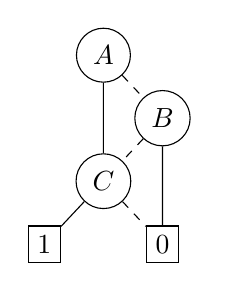
\begin{tikzpicture}[level distance=0.8cm]
      \node[draw,circle] (A) {$A$}
      child {edge from parent[draw=none]}
      child {node[draw,circle] (B) {$B$} edge from parent[dashed]
        child {node[draw,circle,solid] (C) {$C$} edge from parent[dashed]
          child {node[draw,rectangle,solid] {$1$} edge from parent[solid]}
          child {node[draw,rectangle,solid] (0) {$0$}}
        }
        child {edge from parent[draw=none]}
      };
      \draw (A) -- (C);
      \draw (B) -- (0);
    \end{tikzpicture}
    \caption{(RO)BDD}
  \end{subfigure}
  \begin{subfigure}{0.30\textwidth}
    \centering
    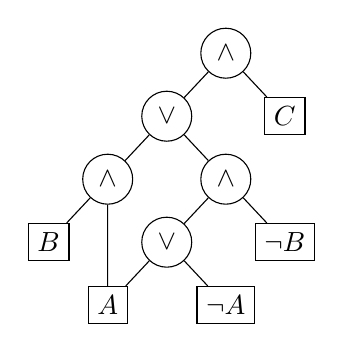
\begin{tikzpicture}[level distance=0.8cm]
      \node[draw,circle] {$\land$}
      child {node[draw,circle] {$\lor$}
        child {node[draw,circle] (parent) {$\land$}
          child {node[draw,rectangle] {$B$}}
          child {edge from parent[draw=none]}
        }
        child {node[draw,circle] {$\land$}
          child {node[draw,circle] {$\lor$}
            child {node[draw,rectangle] (A) {$A$}}
            child {node[draw,rectangle] {$\neg A$}}
          }
          child {node[draw,rectangle] {$\neg B$}}
        }
      }
      child {node[draw,rectangle] {$C$}};
      \draw (parent) -- (A);
    \end{tikzpicture}
    \caption{d-DNNF}
  \end{subfigure}
  \begin{subfigure}{0.30\textwidth}
    \centering
    \begin{tikzpicture}[level distance=0.8cm]
      \tikzset{
        mysplit/.style={
          draw,
          rectangle,
          rectangle split,
          rectangle split horizontal,
          rectangle split parts=2
        }
      }
      \node[draw,circle] {$1$}
      child {node[mysplit] (bullet) {
          \nodepart{one} $\neg A$
          \nodepart{two}
        }
        child {node[draw,circle] (3) {$3$} edge from parent[draw=none]
          child {node[mysplit] {
              \nodepart{one} $\neg B$
              \nodepart{two} $C$
            }
          }
          child {node[mysplit] {
              \nodepart{one} $B$
              \nodepart{two} $\bot$
            }
          }
        }
      }
      child {node[mysplit] {
          \nodepart{one} $A$
          \nodepart{two} $C$
        }};
      \draw[*-] let \p1 = (bullet.two), \p2 = (bullet.center) in ({\x1 + 2.5},{\y2 + 2}) -- (3);
    \end{tikzpicture}
    \caption{SDD}
  \end{subfigure}
  \caption{Example diagrams for $C \land (A \lor \neg B)$}
  \label{fig:kc}
\end{figure}

Many WMC algorithms rely on knowledge compilation, i.e., compilation of the
structure of the initial representation into a form that allows one to perform
various operations and answer queries of interest in time polynomial in the size
of the compiled representation. Traditionally, the initial representation is a
propositional formula. Many such representations have been proposed
\citep{DBLP:journals/jair/DarwicheM02}. Amongst them, the ones that are used in
probabilistic inference include (reduced ordered) binary decision diagrams
((RO)BDDs) \citep{DBLP:journals/tc/Bryant86}, deterministic decomposable negation
normal form (d-DNNF) \citep{DBLP:journals/jancl/Darwiche01}, sentential decision
diagrams (SDDs) \citep{DBLP:conf/ijcai/Darwiche11}, and probabilistic SDDs
\citep{DBLP:conf/kr/KisaBCD14}---some of them are pictured in \cref{fig:kc}. A
BDD is similar to a decision tree that ends with either one or zero but
generalised to a directed acyclic graph. Both d-DNNF and SDD are normal forms
for propositional formulae that satisfy certain properties. Probabilistic SDDs
extend SDDs with probability labels on edges. BDDs are a strict subset of SDDs
that are a strict subset of d-DNNF \citep{DBLP:conf/ijcai/Darwiche11}.

Similarly to how BDDs represent Boolean functions, ADDs represent pseudo-Boolean
functions, i.e., while (non-trivial) BDDs always have two sinks marked with one
and zero, ADDs can have any number of sinks that contain, typically, real
numbers \citep{DBLP:journals/fmsd/BaharFGHMPS97}. ADDs have been extended to
represent the additive and multiplicative structure in sink values more
compactly \citep{DBLP:conf/ijcai/SannerM05} and to support first-order logic
\citep{DBLP:journals/ai/SannerB09} and continuous variables
\citep{DBLP:conf/uai/SannerDB11}. ADDs have been used to represent MDP value
functions \citep{DBLP:conf/uai/HoeySHB99} and probabilities in PGMs
\citep{DBLP:conf/ijcai/ChaviraD07,DBLP:conf/uai/GogateD11}.

\begin{itemize}
\item Boolean and Pseudo-Boolean Functions
\item NNF
\item d-DNNF
\item SDDs
\item BDDs
\item ADDs (with a brief mention of AADDs, XDDs, etc.)
\end{itemize}

\section{Applications}

of WMC?

copy info from my year 2 report

\begin{itemize}
\item Statistical Relational Learning
\item Neuro-Symbolic Artificial Intelligence
\item Natural Language Processing
\item Robotics
\end{itemize}
